\chapter{Background}\label{chap:background}

The following will provide an introduction into some of the core concepts necessary to understand how Polish cryptologists were able to break Enigma in 1932. We will introduce the hardware of the Enigma machine, as well as provide a brief overview of permutation theory. We will also prove a theorem which is integral in creating the permutations used in the set of equations that model the electrical circuit inside Enigma.

\section{Enigma Hardware}

\begin{figure}[h!]
\begin{centering}
  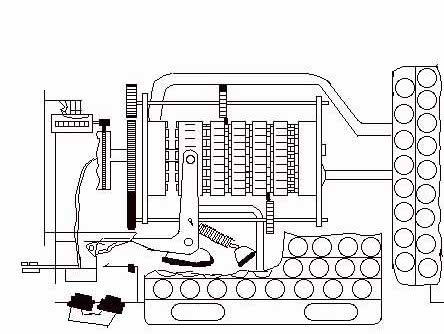
\includegraphics[height=10cm]{images/rotors.jpg}
  \caption{Hardware of the Enigma Machine}
  \label{fig:hardware1}
\end{centering}
\end{figure}

In order to understand how the ciphertexts created by the Enigma machine were broken, it is important to understand the inner workings of the machine itself. Figure \ref{fig:hardware1} shows a schematic of the hardware.

On the outside of each machine, there is a keyboard and a row of glowlamps. Each key on the keyboard is connected to a glowlamp through a changing electric circuit, so when a key is pressed it lights up a corresponding glowlamp. Below the keyboard, there is a plugboard with between six (6) and twelve (12) switches. These switches allow for two letters of the alphabet to be transposed prior to being sent into the machine's hardware. It introduced a "reciprocal monoalphabetic substitution between the keyboard and the first rotor" \cite{bw05}. This adds a layer of security beyond the rotors on the inside of the machine.

Inside each machine, there are anywhere from three (3) to as many as eight (8) rotors and a reflector (or reversing drum). These rotors are the main ciphering components. Each rotor has the alphabet inscribed on the rim, twenty-six (26) fixed contacts on one face, and twenty-six (26) spring loaded contacts on the other face \cite{wk85}. Each rotor has a unique circumference, as well as a unique set of connected contacts. These contacts are randomly connected, and are different on each rotor \cite{bw05}. The reversing drum is responsible for creating the reciprocal nature of the machine, meaning that if an 'A' is pressed on the keyboard and an 'F' lights up on the glow lamps, it also means that if an 'F' is pressed on the keyboard, the 'A' will light up on the glow lamps.

Each rotor inside the machine is set up in such a way that it will rotate corresponding to different key presses. The rotor closest to the keyboard rotates every time a key is pressed, meaning that the substitution changes every time a key is pressed. The other two (2) to seven (7) rotors rotate at variable rates, depending on how the hardware is configured. The second rotor's rotation is dependent on the first rotor's rotation, the third rotor is dependent on the second, and so on and so forth. This rotation of the rotors adds another level of complexity on top of the already complex substitution cipher that Enigma creates.

\section{Important Mathematical Concepts}
- permutations
- proof (theorem of product of transpositions)
